\documentclass[11pt, fleqn]{article}

\documentclass[11pt, fleqn]{article}

\usepackage[usenames,dvipsnames,svgnames,table]{xcolor}
\usepackage{amsmath}
\usepackage{amsfonts}
\usepackage[margin=1in]{geometry} % To set the margin widths
\usepackage{graphicx}
\usepackage{listings}
\usepackage{multirow}
\usepackage{tabularx}
\usepackage{varioref}
\usepackage[noabbrev,capitalize]{cleveref}
\usepackage[group-separator={,}]{siunitx}
\usepackage{subcaption}
\usepackage{titlesec}
\usepackage{lscape}
\usepackage{bm}
\usepackage[titletoc,toc,title]{appendix}

\lstset{
  frame=single,
  basicstyle=\ttfamily,% print whole listing small
  language=R,
  aboveskip=3mm,
  belowskip=3mm,
  showstringspaces=false,
  columns=flexible,
  numbers=none,
  commentstyle=\color{ForestGreen},
  stringstyle=\color{Maroon},
  breaklines=true,
  breakatwhitespace=true,
  tabsize=2,
  literate={<-}{{$\gets$}}1 {~}{{$\sim$}}1
}

\sisetup{output-exponent-marker=\textsc{e}}

\setlength{\parskip}{12pt} % Sets a blank line in between paragraphs
\setlength\parindent{0pt} % Sets the indent for each paragraph to zero

% \crefname{figure}{Figure}{Figures}
% \crefname{section}{Section}{Sections}
% \crefname{table}{Table}{Tables}
% \crefname{lstlisting}{Listing}{Listings}

\setlength{\parskip}{12pt} % Sets a blank line in between paragraphs
\setlength\parindent{0pt} % Sets the indent for each paragraph to zero

\begin{document}

\title{Machine Learning (41204-01)\\HW \#3}
\author{Will Clark $\vert$ Matthew DeLio \\
\texttt{will.clark@chicagobooth.edu} $\vert$ \texttt{mdelio@chicagobooth.edu} \\
University of Chicago Booth School of Business}
\date{\today}
\maketitle

% Describe the data, show a plot of mileage vs price

\section{Data Description}

The data set for this exercise is the sale price and observed mileage for 1000 used cars of what appear to be the same make/model. We can see in \cref{fig:linear} that the expected inverse relationship between mileage and sale price is borne out by the data (i.e. high-mileage cars are less expensive than low-mileage cars).

\section{Linear Regression Model}\label{sec:linear}

To describe this data, we first estimate a linear model of mileage on price:
\[ p_i = \alpha + \beta m_i + \varepsilon_i \]
where \(p_i\) is the price of car \(i\), \(m_i\) is the observed mileage on car \(i\), \(\alpha\) and \(\beta\) are estimated regression coefficients, and \(\varepsilon_i\) is the residual. We fit a generalized linear model to the data and find that \(\alpha=56359.7\) and \(\beta=-0.35\). That is, a hypothetical used car with no miles would sell for about \$56 thousand, and each additional mile driven lowers a car's expected selling price by \$0.35.

As depicted in \cref{fig:linear}, this model appears to be a weak fit for the data (i.e. the residuals are not normally distributed). The model tends to systematically under-value cars with very low mileage and with very high mileage (see \cref{fig:lin_errors} in the Appendix). 

\begin{figure}[!htb]
  \centering
  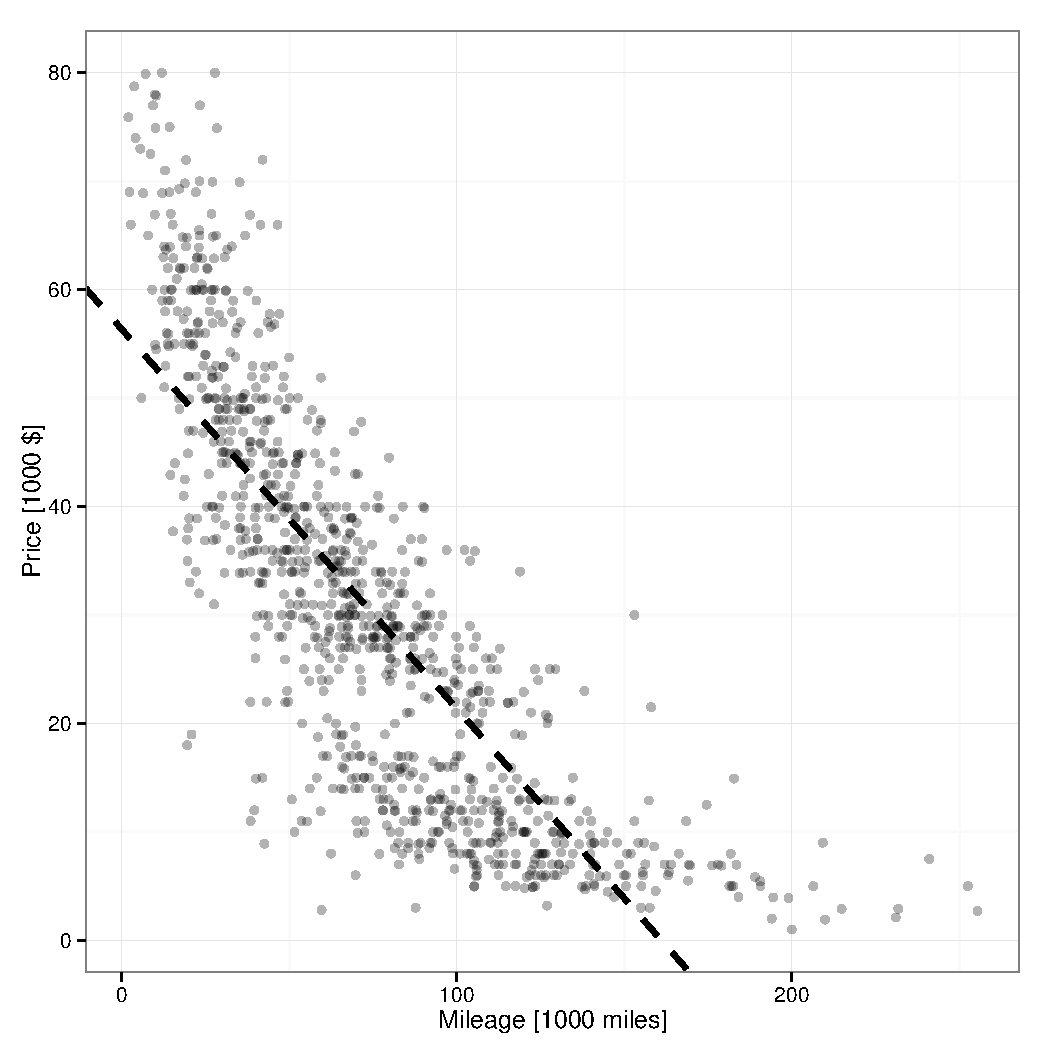
\includegraphics[scale=.5]{linear_fit.pdf}
  \caption{Linear Regression of Price on Mileage}
  \label{fig:linear}
\end{figure}

\section{k-Nearest Neighbors Algorithm}

As an alternative to a linear model, we consider the use of a k-nearest neighbors (kNN) algorithm. This algorithm computes an expected price for every given mileage by taking an average of the observed price for the k-number of cars with the closest observed mileage. 

The decision we are faced with is choosing a value for the k-number of nearest neighbors to include in the algorithm. There are many different decision criteria we could use, but we will focus on two: 1) out-of-sample root mean square error (RMSE); and 2) n-fold cross-validation (CV).

\subsection{Out-of-Sample RMSE}\label{sec:oos}

To choose $k$ using out-of-sample RMSE, we break our data into a training sample (with 900 data points) to train a model, and a test sample (with the remaining 100 points) to estimate the model's goodness of fit. We then estimate a model for all integer values of $k \in (2,100)$ and compare their out-of-sample RMSEs, where RMSE is defined by:
\[ \text{RMSE} = \sqrt{\frac{1}{n} \sum_{i=1}^{n} \left( p_i - \hat{p_i} \right)^2} \]

where $p_i$ is the observed price of car $i$ and $\hat{p_i}$ is the predicted price of car $i$ given its mileage. The RMSE is a measure of how closely a model fits the data; in this case, what we care about is how well the model fits data points that it has not been trained on. We then choose the $k$ that produces the lowest out-of-sample RMSE. The results are depicted in \cref{fig:sweep} (in the red line). We can see that the minimum RMSE occurs at $k=12$, which is circled in the plot.\footnote{The value of $k$ selected depends heavily on the hold-out sample, which is selected randomly. We manually seeded R's random number generator for this example, but letting it vary produces very different values of $k$ fluctuating around the optimal cross-validated $k$ found in next section.}

% use n-fold cross-validation
\subsection{n-fold Cross Validation}\label{sec:cv}

The alternative method is to choose $k$ via cross validation. In this method, we measure out-of-sample fit using the same method as in the prior section (via RMSE), but, instead, we average the out-of-sample fit of ten different training sets (i.e. n-fold cross-validation with $n=10$). The algorithm, briefly:
\begin{itemize}
\item For all $k \in (2,100)$:
\begin{itemize}
\item Break the sample into 10 different data sets
\item For all $n \in (1, 10)$:
\begin{itemize}
\item Hold out the $n$-th data set; train a model on the remaining data
\item Calculate the RMSE of the $n$-th (held out) data set based on the predicted values of the k-nn model
\end{itemize}
\item Each $k$ will have $n$ RMSE values; take the average of all these RMSEs.
\end{itemize}
\item Select the model ($k$) with the lowest average RMSE (which we will call cross-validated error).
\end{itemize}

The resulting RMSE for various values of k is shown in \cref{fig:sweep} (the light blue line). The choice of $k$ that results in the lowest cross-validated error is $k=40$, which is circled in blue in the figure.\footnote{As a comparison, using the \texttt{kknn} package's built-in algorithm for hold-one-out cross-validation selects a model with $k=41$, so our result is close to optimal.}

\begin{figure}[!htb]
  \centering
  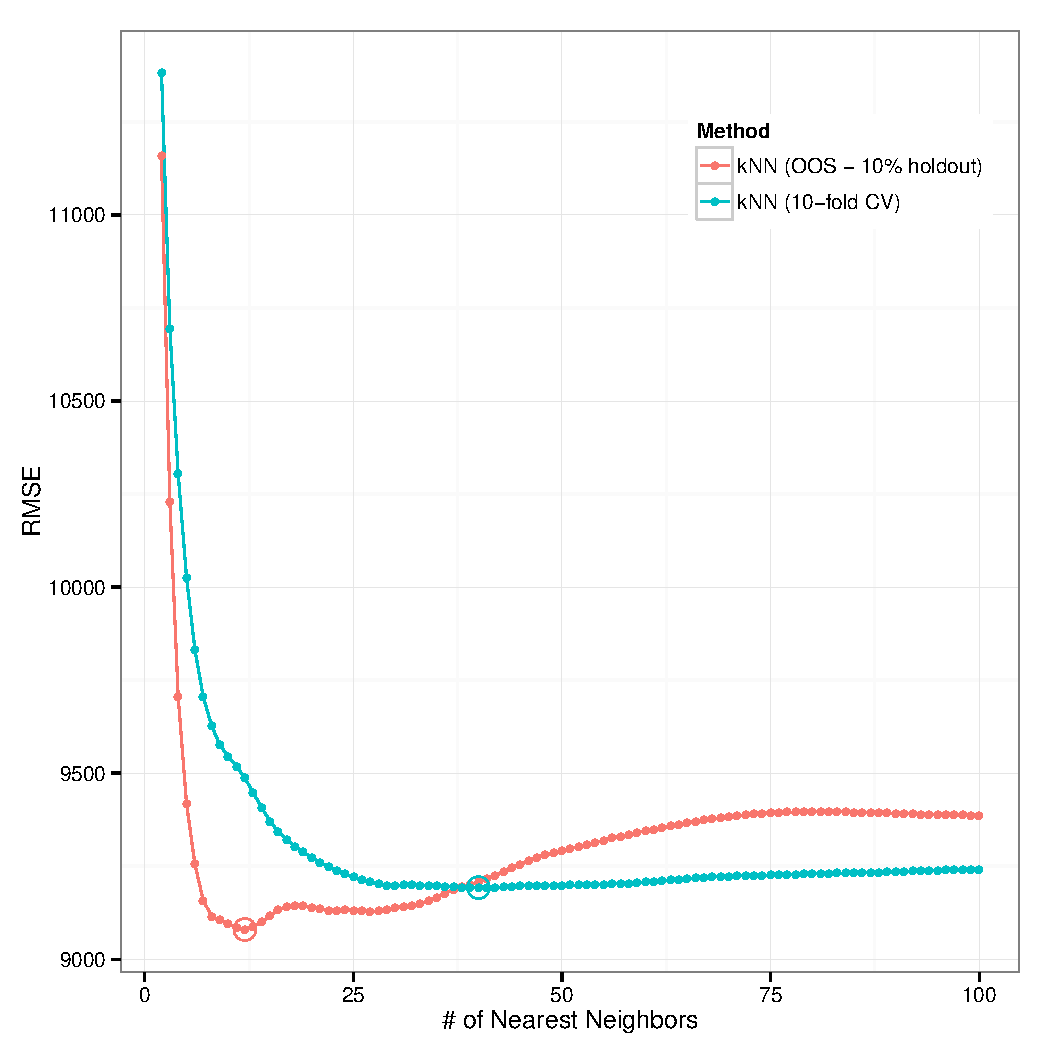
\includegraphics[scale=.5]{sweep_kknn.pdf}
  \caption{CV and OOS RMSE for Various Values of k in kNN}
  \label{fig:sweep}
\end{figure}

\section{Model Predictions}

Before making any predictions we first compare the linear model found in \cref{sec:linear} to the ones developed in \cref{sec:oos,sec:cv}.  We make a comparison of the algorithms using \cref{fig:models} to see how they visually track the car pricing data.  In addition to showing the linear model's fit, we show how the kNN algorithm tracks with a low value of $k=12$ (the one indicated in \cref{sec:oos}), a medium one at $k=40$ (prescribed through the cross-validation method from \cref{sec:cv}), and finally one with $k=500$ (a arbitrary and unreasonably large choice).

These three values illustrate the Bias-Variance trade-off clearly.  For our small value of $k=12$, kNN tracks the data closely but also tends to latch onto variance in the data (seen as tracking jitter).  On the other side of the spectrum, as $k$ increases to an unreasonably large value of $k=500$ it tends to ignore the variance (it's smooth), but introduces a large amount of bias (mispredicting greatly at higher mileages).  Our prior work indicated that $k=40$ would achieve a good trade-off where the algorithm could still track the data well, without introducing too much bias and without tracking too much variance as well.  Indeed we see that this choice yields a much smoother line than $k=12$ and introduces no noticeable bias.

\begin{figure}[!htb]
  \centering
  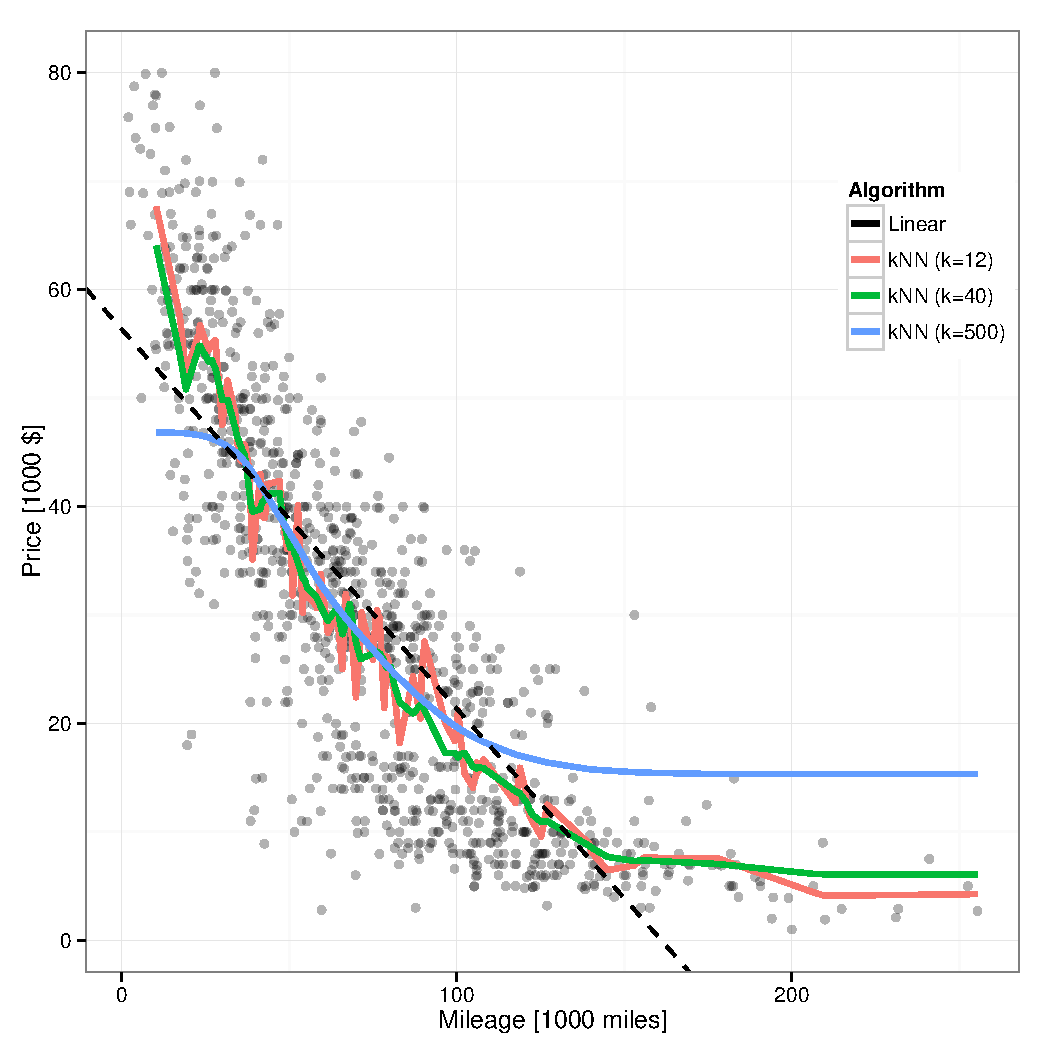
\includegraphics[scale=.5]{pred_models.pdf}
  \caption{Comparison of Models Created by the Linear and kNN}
  \label{fig:models}
\end{figure}

For a more quantitative comparison of these models we turn to, \cref{tab:rmse_compare}.\footnote{This comparison uses the same training/test sample described in \cref{sec:oos}}  Here it is immediately evident that the Linear and $k=500$ algorithms exhibit the worse RSME's.  For the better two, $k=12$ and $k=40$, it appears as though the $k=12$ model slightly beats $k=40$.  However, as pointed out in previous sections the 10-fold cross-validated value of $k=40$ is likely a better parameter choice for out-of-sample predictions and will be used for the remainder of this section.

% latex table generated in R 3.1.2 by xtable 1.7-4 package
% Wed Sep 30 22:12:10 2015
\begin{table}[ht]
\centering
\begin{tabular}{rr}
  \hline
 & RMSE \\ 
  \hline
Linear & 23616.73 \\ 
  kNN ($k=12$) & 9079.60 \\ 
  kNN ($k=40$) & 9206.86 \\ 
  kNN ($k=500$) & 10636.19 \\ 
   \hline
\end{tabular}
\caption{Comparison of RMSEs} 
\label{tab:rmse_compare}
\end{table}


With our algorithm (kNN) and parameter ($k=40$) chosen, we then use compare the predictions of the linear model and kNN algorithm for a car with 100,000 miles.  At this mileage, the linear model predicts that the car's value is \$21,362.33 while the kNN model predicts \$17,936.67 (these predictions are shown as colored circles in \cref{fig:predict}).  Examining this figure further, the mass of cars priced below \$20,000 with roughly 100,000 miles give us more confidence in kNN over the linear model.

% > preds
%   mileage linear.pred knn.pred
% 1   1e+05    21362.33 17936.67

\begin{figure}[!htb]
  \centering
  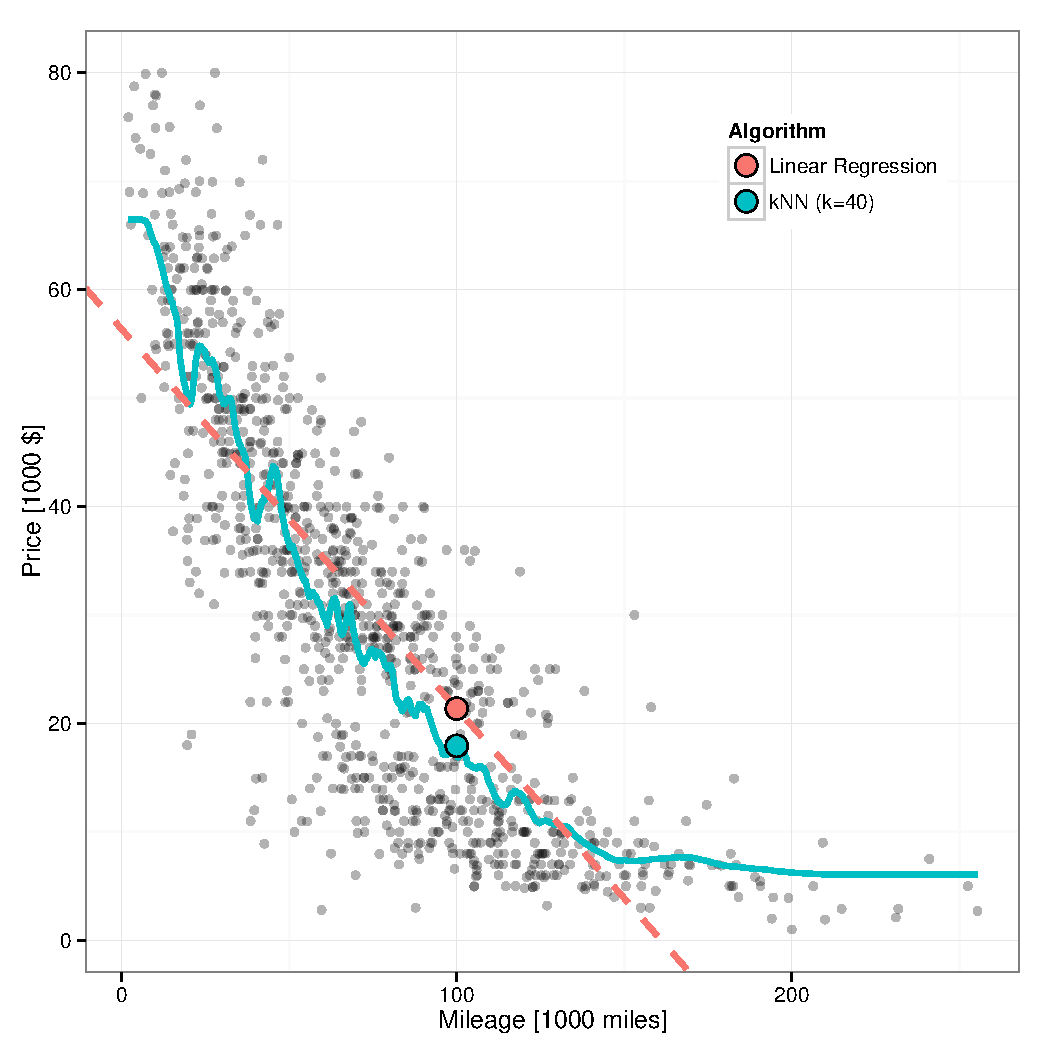
\includegraphics[scale=.5]{predict.pdf}
  \caption{Linear \& kNN Predictions}
  \label{fig:predict}
\end{figure}

\clearpage
\section{Appendix}

\begin{figure}[!htb]
  \centering
  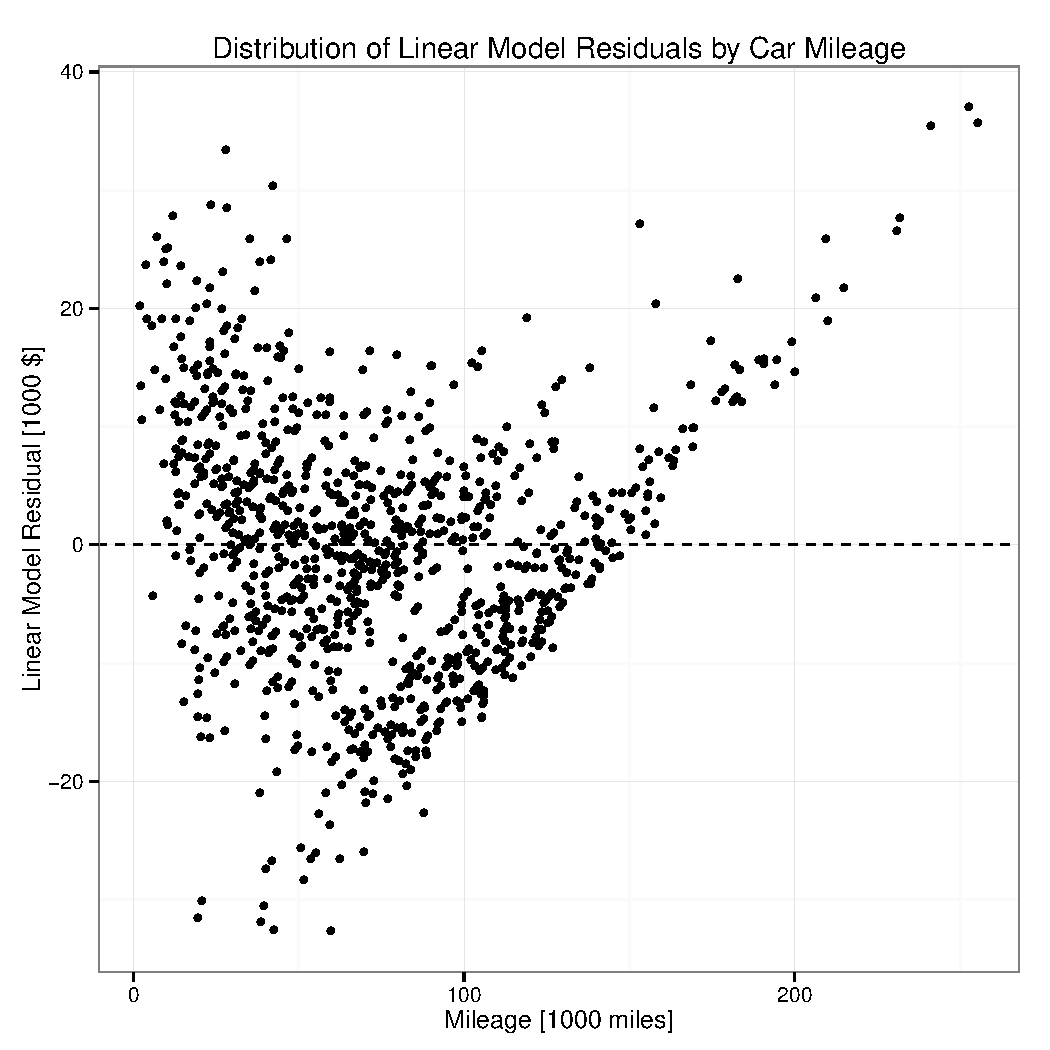
\includegraphics[scale=.5]{lin_errors.pdf}
  \caption{Distribution of Residuals in Linear Model}
  \label{fig:lin_errors}
\end{figure}

\end{document}

% \input{.tex}

% \begin{figure}
%   \centering
%   \begin{subfigure}[b]{0.49\textwidth}
%     \includegraphics[width=\textwidth]{.pdf}
%     \caption{}
%     \label{fig:}
%   \end{subfigure}
%   \hfill
%   \begin{subfigure}[b]{0.49\textwidth}
%     \includegraphics[width=\textwidth]{.pdf}
%     \caption{}
%     \label{fig:}
%   \end{subfigure}
%   \caption{}
% \end{figure}

% \begin{figure}[!htb]
%   \centering
%   \includegraphics[scale=.5]{.pdf}
%   \caption{}
%   \label{fig:}
% \end{figure}

